\documentclass{article}
\usepackage[utf8]{inputenc}
\usepackage[vietnamese, main=english]{babel}
\usepackage{graphicx}

\begin{document}
\begin{titlepage}
	\title{
		\Large{Distributed System - Practical work 1} \\
		\Huge{\textbf{TCP File transfer}} \\
		\includegraphics[width=0.4\textwidth]{logo-usth-pa3-01.png}
	}
	\author{
		\selectlanguage{vietnamese} Ngô Ngọc Đức Huy -- BI9-119 \\
	}
	\date{\today}
\end{titlepage}

\maketitle

\section{Protocol}

We modify the provided simple chat system to make this file transfering system.
In this proof-of-concept we only concerns the file sending from the client to the server.

After the initial request for connection being accepted, the client sends to the server
the file's metadata:

\begin{itemize}
	\item file size, so that the server knows how many packets to receive
	\item file name, so that the server knows what to save as
\end{itemize}

The client consequently sends chunks of data until all the file is sent.
After that, it prompts to disconnect with the server.

\begin{figure}
	\centering
	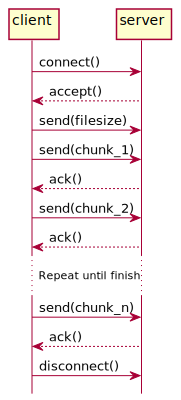
\includegraphics{pw1/protocol.pdf}
	\caption{Our protocol for file transfering}
\end{figure}

\section{System organization}

In this system, the client and the server each has a program dedicated for sending or receiving
and a file system. The sender program reads the file at the client and send it to the server
using TCP/IP protocol. The receiver program at the server writes to a file upon receiving the data.

\begin{figure}
	\centering
	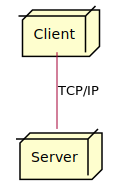
\includegraphics{pw1/system-org.pdf}
	\caption{The system organization}
\end{figure}

\section{Implementation}



\end{document}
